\pdfminorversion=4
\documentclass[aspectratio=169]{beamer}

\mode<presentation>
{
  \usetheme{default}
  \usecolortheme{default}
  \usefonttheme{default}
  \setbeamertemplate{navigation symbols}{}
  \setbeamertemplate{caption}[numbered]
  \setbeamertemplate{footline}[frame number]  % or "page number"
  \setbeamercolor{frametitle}{fg=white}
  \setbeamercolor{footline}{fg=black}
} 

\usepackage[english]{babel}
\usepackage[utf8x]{inputenc}
\usepackage{tikz}
\usepackage{courier}
\usepackage{array}
\usepackage{bold-extra}
\usepackage{minted}
\usepackage[thicklines]{cancel}
\usepackage{fancyvrb}

\xdefinecolor{dianablue}{rgb}{0.18,0.24,0.31}
\xdefinecolor{darkblue}{rgb}{0.1,0.1,0.7}
\xdefinecolor{darkgreen}{rgb}{0,0.5,0}
\xdefinecolor{darkgrey}{rgb}{0.35,0.35,0.35}
\xdefinecolor{darkorange}{rgb}{0.8,0.5,0}
\xdefinecolor{darkred}{rgb}{0.7,0,0}
\definecolor{darkgreen}{rgb}{0,0.6,0}
\definecolor{mauve}{rgb}{0.58,0,0.82}

\title[2018-10-01-dianahep-histbook]{Histogram interoperability}
\author{Jim Pivarski}
\institute{Princeton University -- DIANA-HEP}
\date{October 1, 2018}

\usetikzlibrary{shapes.callouts}

\begin{document}

\logo{\pgfputat{\pgfxy(0.11, 7.4)}{\pgfbox[right,base]{\tikz{\filldraw[fill=dianablue, draw=none] (0 cm, 0 cm) rectangle (50 cm, 1 cm);}\mbox{\hspace{-8 cm}
\includegraphics[height=1 cm]{princeton-logo-long.png}
\includegraphics[height=1 cm]{diana-hep-logo-long.png}}}}}

\begin{frame}
  \titlepage
\end{frame}

\logo{\pgfputat{\pgfxy(0.11, 7.4)}{\pgfbox[right,base]{\tikz{\filldraw[fill=dianablue, draw=none] (0 cm, 0 cm) rectangle (50 cm, 1 cm);}\mbox{\hspace{-8 cm}
\includegraphics[height=1 cm]{princeton-logo.png}
\includegraphics[height=1 cm]{diana-hep-logo.png}}}}}

% Uncomment these lines for an automatically generated outline.
%\begin{frame}{Outline}
%  \tableofcontents
%\end{frame}

% START START START START START START START START START START START START START

\begin{frame}{Histogramming in Python}
\scriptsize
\vspace{0.25 cm}
\begin{columns}
\column{1.1\linewidth}
\renewcommand{\arraystretch}{1.2}
\begin{tabular}{c l c p{2.7 cm} p{1.5 cm} p{4.75 cm}}
pip? & name & last release & interface style & depends on & integrates with \\\hline
& \href{https://root.cern.ch/pyroot}{\textcolor{blue}{PyROOT}} & 2018 & HEP & ROOT & numpy \\
& \href{https://yoda.hepforge.org/pydoc}{\textcolor{blue}{YODA}} & 2018 & HEP & {\it compiled} & matplotlib, yaml \\
$\surd$ & \href{https://pypi.python.org/pypi/physt}{\textcolor{blue}{physt}} & 2018 & HEP + data science & numpy & pandas, xarray, dask, protobuf, matplotlib, vega (plotting), folium (maps) \\
$\surd$ & \href{https://pypi.org/project/fast-histogram}{\textcolor{blue}{fast-histogram}} & 2018 & simple (astronomy) & numpy & \\
$\surd$ & \href{https://pypi.org/project/qhist/}{\textcolor{blue}{qhist}} & 2018 & HEP & ROOT & \\
$\surd$ & \href{https://pypi.org/project/rootpy}{\textcolor{blue}{rootpy}} & 2017 & HEP & ROOT & pytables, matplotlib, stats \\
$\surd$ & \href{https://vaex.io}{\textcolor{blue}{Vaex}} (vaex.io) & 2017 & all-in-one GUI for big data, fast heatmaps & {\it many!} & Jupyter, matplotlib, HDF5, pandas, C++ \\
$\surd$ & \href{https://pypi.python.org/pypi/hdrhistogram}{\textcolor{blue}{hdrhistogram}} & 2017 & ``high dynamic range'' & {\it compiled} & Java, C++ \\
$\surd$ & \href{https://pypi.python.org/pypi/multihist}{\textcolor{blue}{multihist}} & 2017 & numpy wrapper & numpy & matplotlib \\
$\surd$ & \href{https://github.com/ibab/matplotlib-hep}{\textcolor{blue}{matplotlib-hep}} & 2016 & HEP & matplotlib & numpy, scipy \\
$\surd$ & \href{https://pypi.python.org/pypi/pyhistogram}{\textcolor{blue}{pyhistogram}} & 2014 & HEP & numpy & matplotlib, datetime \\
$\surd$ & \href{https://pypi.python.org/pypi/histogram}{\textcolor{blue}{histogram}} & 2011 & HEP & numpy & matplotlib, HDF5 \\
$\surd$ & \href{https://pypi.python.org/pypi/SimpleHist}{\textcolor{blue}{SimpleHist}} & 2011 & HEP & numpy, matplotlib & ROOT \\
$\surd$ & \href{https://pypi.org/project/paida}{\textcolor{blue}{paida}} & 2007 & HEP & & AIDA! \\
& \href{https://github.com/theodoregoetz/histogram}{\textcolor{blue}{theodoregoetz}} & never & HEP & scipy, \mbox{uncertainties} & numpy, matplotlib \\
% $\surd$ & \href{https://pypi.python.org/pypi/histogramy}{\textcolor{blue}{histogramy}} & 2013 & Numpy, Matplotlib, Scikit-Learn & & \\
% $\surd$ & \href{https://pypi.python.org/pypi/pypeaks}{\textcolor{blue}{pypeaks}} & 2014 & & & \\
% $\surd$ & \href{https://pypi.python.org/pypi/hierogram}{\textcolor{blue}{hierogram}} & 2014 & & & \\
% $\surd$ & \href{https://pypi.python.org/pypi/histo}{\textcolor{blue}{histo}} & & & & \\
% $\surd$ & \href{https://pypi.python.org/pypi/python-metrics}{\textcolor{blue}{python-metrics}} & & & & \\
% $\surd$ & \href{https://pypi.python.org/pypi/statscounter}{\textcolor{blue}{statscounter}} & 2016 & & & \\
% $\surd$ & \href{https://pypi.python.org/pypi/datagram}{\textcolor{blue}{datagram}} & & & & \\
% & \href{http://www.ifh.de/~middell/dashi/index.html}{\textcolor{blue}{dashi}} & & & & \\
\end{tabular}
\end{columns}
\end{frame}

\begin{frame}{Over the years, I've written five}
\scriptsize
\vspace{0.25 cm}
\begin{columns}
\column{1.1\linewidth}
\renewcommand{\arraystretch}{1.2}
\begin{tabular}{c l c p{2.7 cm} p{1.5 cm} p{4.75 cm}}
pip? & name & last release & interface style & depends on & integrates with \\\hline
& \href{http://code.google.com/p/plothon}{\textcolor{blue}{Plothon}} & 2006 & HEP & ROOT & SVG \\
& \href{http://code.google.com/p/svgfig}{\textcolor{blue}{SVGFig}} & 2008 & HEP & {\it none!} & SVG \\
& \href{https://github.com/opendatagroup/cassius}{\textcolor{blue}{Cassius}} & 2013 & HEP + data science & numpy & SVG, Augustus (Open Data Group) \\
$\surd$ & \href{https://github.com/histogrammar}{\textcolor{blue}{Histogrammar}} & 2016 & combinational library & numpy & Spark, Julia, CUDA, \mbox{ROOT (Cling),} matplotlib, Bokeh, Vega \\
$\surd$ & \href{https://github.com/scikit-hep/histbook}{\textcolor{blue}{histbook}} & 2018 & HEP & numpy & Spark, Pandas, Vega \\
\end{tabular}
\end{columns}

\large
\begin{uncoverenv}<2->
\vspace{1 cm}
\underline{\it Implementing} data analysis tools isn't the problem, it's designing the \underline{\it right} tool, one that solves the Cuisinart Problem:

\begin{center}
\begin{minipage}{0.8\linewidth}
It slices and dices, but is it worth the setup and cleanup?
\end{minipage}
\end{center}

Experimentation in this area is valuable.
\end{uncoverenv}
\end{frame}

\begin{frame}{All these libraries are overwhelming!}
\large
\vspace{0.5 cm}
\begin{center}

\includegraphics[width=0.4\linewidth]{standards.png}
\end{center}

\vspace{0.5 cm}
However, the real problem isn't data analysts using different tools; the problem is communicating results between data analysts.
\end{frame}

\begin{frame}{There is a standard: ROOT files}
\large
\vspace{0.5 cm}
Even if the point of a tool is to work in a non-ROOT way or to avoid ROOT dependencies, we can still share results in the ROOT file format.

\vspace{1 cm}
\textcolor{darkblue}{Look at industry:}
\begin{itemize}
\item dozens of big data SQL engines that all run on Parquet files;
\item dozens of machine learning tools that all run on Numpy from HDF5 files.
\end{itemize}

\vspace{0.25 cm}
The most conservative part of a software ecosystem is its persistence format.

\vspace{1 cm}
ROOT files are incredibly well established in HEP. It would take a strong technical argument/corner case to use something else.
\end{frame}

\begin{frame}[fragile]{Writing histograms with uproot}
\large
\vspace{0.5 cm}
uproot version 3 has write support, but (currently) only for histograms.

\small
\begin{minted}{python}
>>> import uproot
>>> import numpy
>>> f = uproot.recreate("tmp.root")
>>> f["name"] = numpy.histogram(numpy.random.normal(0, 1, 100000))
\end{minted}

\vspace{1 cm}
\large
Read it back in ROOT:

\small
\begin{minted}{python}
>>> import ROOT
>>> f = ROOT.TFile("tmp.root")
>>> h = f.Get("name")
>>> h.Draw()
\end{minted}

\vspace{-3.5 cm}
\hfill 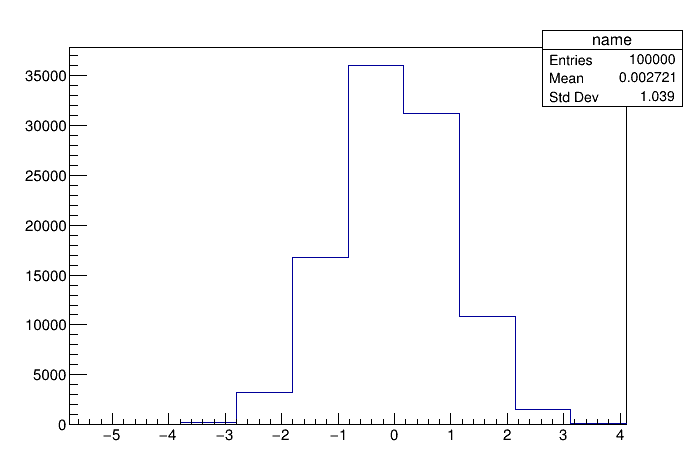
\includegraphics[width=0.5\linewidth]{root-hist.png}
\end{frame}

\begin{frame}[fragile]{Bidirectional conversions to and from many libraries}
\vspace{0.1 cm}
\normalsize
Save a Physt plot to a ROOT file:

\small
\begin{minted}{python}
>>> import physt
>>> f = uproot.recreate("tmp.root")
>>> f["name"] = physt.h1(numpy.random.normal(0, 1, 100000), bins=16,
...                      range=(-4, 4), name="physt histogram")
\end{minted}

\normalsize
Read it back as Physt:

\small
\begin{minted}{python}
>>> f["name"].physt().plot()
\end{minted}

\normalsize
Read it back as a Numpy contents-and-edges tuple:

\small
\begin{minted}{python}
>>> f["name"].numpy()
\end{minted}

\tiny
\begin{verbatim}
(array([   23,   112,   473,  1652,  4370,  9061, 15024, 19213, 19091, 15019,  9128,  4501,  1671,   512,   128,    16], dtype=int32),
 array([-4. , -3.5, -3. , -2.5, -2. , -1.5, -1. , -0.5,  0. ,  0.5,  1. ,  1.5,  2. ,  2.5,  3. ,  3.5,  4. ]))
\end{verbatim}

\normalsize
Read it in ROOT:

\small
\begin{minted}{python}
>>> f = ROOT.TFile("tmp.root")
>>> h = f.Get("name")
>>> h.Draw()
\end{minted}
\end{frame}

\begin{frame}[fragile]{Not really ``histograms:'' HEPData archival format (YAML)}
\small
\begin{minted}{python}
>>> print(f["name"].hepdata())
\end{minted}

\tiny
\vspace{-0.6 cm}
\begin{columns}[t]
\column{0.4\linewidth}
\begin{verbatim}
independent_variables:
- header: {name: physt histogram, units: null}
  values:
  - {low: -4.0, high: -3.5}
  - {low: -3.5, high: -3.0}
  - {low: -3.0, high: -2.5}
  - {low: -2.5, high: -2.0}
  - {low: -2.0, high: -1.5}
  - {low: -1.5, high: -1.0}
  - {low: -1.0, high: -0.5}
  - {low: -0.5, high: 0.0}
  - {low: 0.0, high: 0.5}
  - {low: 0.5, high: 1.0}
  - {low: 1.0, high: 1.5}
  - {low: 1.5, high: 2.0}
  - {low: 2.0, high: 2.5}
  - {low: 2.5, high: 3.0}
  - {low: 3.0, high: 3.5}
  - {low: 3.5, high: 4.0}
dependent_variables:
- header: {name: counts, units: null}
  qualifiers: []
  values:
  - value: 23.0
    errors:
    - {symerror: 4.795831523312719, label: stat}
  - value: 112.0
    errors:
    - {symerror: 10.583005244258363, label: stat}
\end{verbatim}
\column{0.5\linewidth}
\begin{verbatim}
  - value: 473.0
    errors:
    - {symerror: 21.748563170931547, label: stat}
  - value: 1652.0
    errors:
    - {symerror: 40.64480286580315, label: stat}
  - value: 4370.0
    errors:
    - {symerror: 66.10597552415364, label: stat}
  - value: 9061.0
    errors:
    - {symerror: 95.1892851112981, label: stat}
  - value: 15024.0
    errors:
    - {symerror: 122.5724275683565, label: stat}
  - value: 19213.0
    errors:
    - {symerror: 138.61096637712328, label: stat}
  - value: 19091.0
    errors:
    - {symerror: 138.17018491700733, label: stat}
  - value: 15019.0
    errors:
    - {symerror: 122.55202976695246, label: stat}
  - value: 9128.0
    errors:
    - {symerror: 95.5405672999695, label: stat}
  - value: 4501.0
    errors:
    - {symerror: 67.08949247087803, label: stat}
  - value: 1671.0
    errors:
    - {symerror: 40.87786687193939, label: stat}
  - value: 512.0
    errors:
    - {symerror: 22.627416997969522, label: stat}
  - value: 128.0
    errors:
    - {symerror: 11.313708498984761, label: stat}
  - value: 16.0
    errors:
    - {symerror: 4.0, label: stat}
\end{verbatim}
\end{columns}
\end{frame}

\begin{frame}[fragile]{Not really ``histograms:'' Pandas DataFrame}
\large

\begin{columns}[b]
\column{0.4\linewidth}
\small
\begin{minted}{python}
>>> f["name"].pandas()
\end{minted}

\scriptsize
\begin{verbatim}
                 count  variance
physt histogram
[-inf, -4.0)         5         5
[-4.0, -3.5)        23        23
[-3.5, -3.0)       112       112
[-3.0, -2.5)       473       473
[-2.5, -2.0)      1652      1652
[-2.0, -1.5)      4370      4370
[-1.5, -1.0)      9061      9061
[-1.0, -0.5)     15024     15024
[-0.5, 0.0)      19213     19213
[0.0, 0.5)       19091     19091
[0.5, 1.0)       15019     15019
[1.0, 1.5)        9128      9128
[1.5, 2.0)        4501      4501
[2.0, 2.5)        1671      1671
[2.5, 3.0)         512       512
[3.0, 3.5)         128       128
[3.5, 4.0)          16        16
[4.0, inf)           1         1
\end{verbatim}

\column{0.45\linewidth}
The index for this DataFrame is an {\tt\normalsize IntervalIndex}.

\vspace{0.5 cm}
The {\tt\normalsize variance} column is the ``sumw2'' (identical to count when filled without weights).

\vspace{0.5 cm}
There's room here for profile plots to share the same binning.

\vspace{0.5 cm}
See the F.A.S.T.\ package for CMS: Ben Krikler and Tai Sakuma.

\vspace{0.5 cm}
\end{columns}
\end{frame}

\begin{frame}{We can add more without upsetting uproot}
\large
\vspace{0.5 cm}
The code that understands streamers and how to write a TH1 is in {\bf uproot}.

\vspace{0.5 cm}
The code that understands how to convert to and from other libraries is in {\bf uproot-methods}. We can make changes to {\bf uproot-methods} independently of (and more rapidly than) {\bf uproot}.

\begin{center}
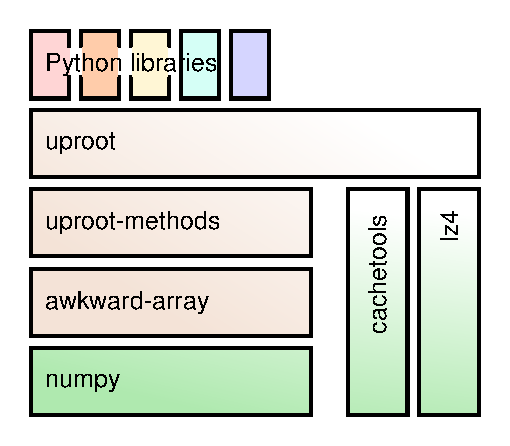
\includegraphics[width=0.4\linewidth]{abstraction-layers.pdf}
\end{center}
\end{frame}


\end{document}
